\chapter{Methodology}
This chapter covers the various methodologies that were implemented in this project, this includes Research methodologies, Software development methodologies, project management, supervisor meetings, developments tools, testing and source control.\newline

An overview of methodologies used in this project;
\textbf{Software development methodologies} which includes Agile Development, Continuous Delivery, Test Driven Development, Feature Driven Development, Extreme Programming etc.
\textbf{Project management} which includes GitHub Kanban board and supervisor meetings.
\textbf{Development tools} Android studio, Firebase.
\textbf{Source Control} GitHub, Overleaf, Badge/Shield

\newpage
\medskip
\section{Project management}
\begin{center}
    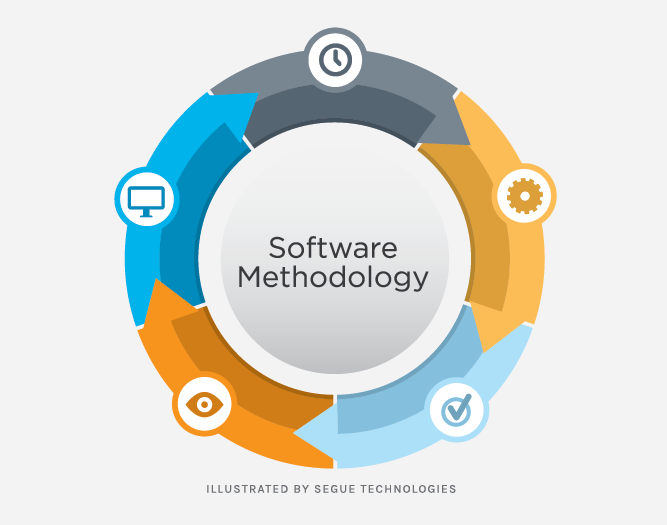
\includegraphics[width=8cm,keepaspectratio]{Images/Software_Method.png}

\end{center}
\par
\par
\medskip
Project Management is a key element of any task to ensure that the project is laid out correctly and each component party is complete at a given date. Because this project is a solo project i used the GitHub Kanban board to first pick features that i may want to implement and then broke them down into separate cards that i could work on individually. This helped brake down tasks which helped in development.

\subsection{Agile}
This project used Agile project management methodologies. An iterative approach was taken. This meant that each week i had certain tasks laid out to be completed be that either a feature for the app or documentation. I also had short weekly/bi-weekly meetings with my supervisor where i would update him, and asks for advice on my dissertation, app, etc. 

\subsubsection{Agile Road-map}
An agile road-map in agile development helps state the goals of the project from the outset. It helps break down the tasks which are then further broken down for sprints. This is usually a high level view of the project. It is used often in industry and it helps to understand a project as a whole and learn what other teams are contributing to the overall project. The roadmap also shows how the project can grow in the future.

\subsubsection{Planning and Development}
During the meeting and planning phase, the milestones \& objectives for the project were identified and broken down into simpler, and more manageable tasks. The tasks are were then grouped into sprints or iterations lasting one to three weeks depending on the task. These are the tasks which mostly completed before each meeting with my supervisor. With each meeting i had a task somewhat completed and i could then know the following task which i could talk with my supervisor about before hand. So each weekly meeting with the supervisor started a sprint and the aim was to complete most of that sprint before the next meeting. The plans for the project and the sprints are taken from the User stories i created on the Kanban project and Design document. Through this iteration i convert the plans into working code.

\subsubsection{Design Phase}
Throughout the agile development life cycle design is a step in every iteration/sprint. The design is gradually built on. The design is never defined at the beginning of the project. The gradual evolution of the design enables taking advantages of new technologies that come on stream as well as meeting any new requirements brought forward by clients. The user experience is key when design a project/application. Every design must be user friendly. The type of end user of the item must be consider when designing. This comes to play in android development often as there is many different tools in development to create different features. You need to test them to know whats best for the end product.

\subsubsection{Testing}
Testing was carried out continuously with Android Studio features. Not only those Android Studio have a huge amount of features the Emulator can test a massive array of devices. So testing for this application was a continuous process throughout every build.

In a real-world environment The user tests would be carried out when meeting with the client. The client using the application would then comment on any changes that should be or could be made.

\section{System Integration}
Producing this project as a solo person meant i used different Software Engineering techniques to development my app. The main approaches used are test driven development(TDD), feature driven development(FDD), and continuous delivery 

\subsection{Test Driven Development}
Test Driven Development is based predominately on unit testing. However they are very different because test driven development is when the unit tests are written before the code has been created. This means the developers are using the unit tests as a gild and the tests alone break down the overall task needing to be completed. The tests will initially fail and the developers write minimal code in order for the tests to pass. This process is continuously repeated in order for the application to pass each test. These tests are commonly automated, in Android Studio a huge amount of testing is automatically completed for you without any manual interference.

\subsection{Feature Driven Development}
Feature Driven Development (FDD) is an agile framework that, as its name suggests, organizes software development around making progress on features. Features in the FDD context, though, are not necessarily product features in the commonly understood sense. They are, rather, more akin to user stories in Scrum. In other words, “complete the login process” might be considered a feature in the Feature Driven Development (FDD) methodology.\cite{FDD}

\subsubsection{FDD planning}
CP prepares iteration planning meeting by grouping the right amount of relevant
features into a work package. Normally the team has a number of CPs, each of them
conducts iterations independently. Each iteration does not have to include the whole 
10 development team. Instead, the new iteration team is formed for each iteration. CP selects
iteration team members based on availability. Each developer receives a subset of
features; strong class ownership is encouraged. The iteration team goes through the list of
features, which should be familiar from Process One. If needed, the team contacts the
customer to clarify any obscure features. In the complex cases the team may create
sequence diagrams. The planning meeting also sets timeline for iteration milestones.\cite{FDD_paper1} \newline
\newpage
\textbf{Lifecycle of FDD}
\begin{enumerate}
  \item \textbf{Develop an overall model} - FDD project starts with high-level walk through of the scope of the system and its context. Next, detailed domain models are created for each modelling area by small groups and presented for peer review.
  \item \textbf{Build a features list} - Knowledge gathered during the initial modeling is used to identify a list of features by functionally decomposing the domain into subject areas. Subject areas each contain business activities, and the steps within each business activity form the basis for a categorized feature list.
  \item \textbf{Plan by feature} - After the feature list is completed, the next step is to produce the development plan and assign ownership of features (or feature sets) as classes to programmers.
  \item \textbf{Design by feature} - A design package is produced for each feature. A chief programmer selects a small group of features that are to be developed within two weeks. Together with the corresponding class owners, the chief programmer works out detailed sequence diagrams for each feature and refines the overall model. Next, the class and method prologues are written and finally a design inspection is held.
  \item \textbf{Build by feature} - After a successful design inspection for each activity to produce a feature is planned, the class owners develop code for their classes. After unit testing and successful code inspection, the completed feature is promoted to the main build.
\end{enumerate}

\subsubsection{Coding in FDD}
Coding process in FDD is not as exciting and challenging as it is in XP. This happens because by the coding time the features have been extensively discussed during Process One, iteration kick-off meeting, design review meeting. Classes and methods are 13 defined by now, their purpose is described in code documentation. Coding often becomes a mechanical process. Unlike XP FDD strongly discourages refactoring. The main argument against refactoring here is that it takes time and does not bring any value to the customer. The quality of code is addressed during code review meetings. FDD encourages strong code ownership. The main idea is that every developer knows the owned code and better realizes the consequence of changes.\cite{FDD_paper1} 
FDD fights the problem of leaving team members from the different angle:
\begin{itemize}
    \item Sufficient code documentation simplifies understanding somebody else’s code
    \item Developers know what other people’s code does, since they reviewed the design
    \item Developers will look at each other’s code during code review
\end{itemize}

\subsection{Continuous Delivery}
Continuous delivery is an extension of continuous integration to make sure that you can release new changes to your customers quickly in a sustainable way. This means that on top of having automated your testing, you also have automated your release process and you can deploy your application at any point of time by clicking on a button.
In theory, with continuous delivery, you can decide to release daily, weekly, fortnightly, or whatever suits your business requirements. However, if you truly want to get the benefits of continuous delivery, you should deploy to production as early as possible to make sure that you release small batches that are easy to troubleshoot in case of a problem. \cite{Cont_delivery_2}

\subsubsection{Continuous Delivery in an Android Environment}

In the context of mobile development, Continuous Delivery is the ability to produce valid builds that are ready to be published in an app store. Continuous Deployment is the final status of the process, which ensures that any of the changes applied to the code is automatically deployed to the production environment.\newline

Continuous Delivery for mobile development can be tricky. For Android app development requires a key to sign off the production build before it can move to the Google Play Store. Keeping keys and passwords on a Version Control Software (VCS) is a bad practise, because VCS is available to any member with access to the project, which includes any temporary 3rd parties. It's common practise therefore to create release build on a local computer, but this erodes one of the great advantages to Continuous delivery: having a scalable online platform and the ability to easily deploy any stages of the Continuous Integration at any time.\cite{Cont_delivery_1} \newline

Because of this you need to secure the signing keys of the app, building a Continuous Delivery around a mobile development environment can be tricky. For Android app development, you can improve this by implementing \hyperlink{https://developer.android.com/studio/publish/app-signing}{Google Play App Signing}, which applies a second key when your app is uploaded to the Google Play Store. But even after employing this method, there will still be at least a key and a couple passwords required to build a release (signing key, key and upload password). To get past this you can use a Encrypted Cloud Storage service for this problem. They can keep the keys safe and are only limited by the integration capabilities of your chosen Continuous Delivery system.
\newpage
\subsubsection{Implementing Continuous Delivery}
Implementing Continuous Delivery, it requires you pick the right tools for the job. So choosing your Continuous Integration system is important. For this project because i was solo i could just use my local computer for deployment and tool integration inside Android Studio is so good, i didn't need to implement these tools, but in a real-world environment working with a team this implementation is mandatory \newline

\textbf{Some examples of Continuous integration systems:}
\begin{itemize}
    \item \hyperlink{https://docs.gitlab.com/ee/ci/}{GitLab CI}
    \item \hyperlink{https://circleci.com/docs/2.0/about-circleci}{CircleCI}
    \item \hyperlink{https://documentation.codeship.com/basic/quickstart/getting-started}{CodeShip}
    \item \hyperlink{https://github.com/features/actions}{Github Actions}
    \item \hyperlink{https://aws.amazon.com/getting-started/projects/set-up-ci-cd-pipeline}{AWS Pipeline}
\end{itemize}

Using these systems with a Version Control System such as GitHub is an easy feat to accomplish and results in a final system as shown below

\begin{figure}[h!]
	\caption{Continuous Delivery Setup for an Android App \cite{Cont_delivery_1}}
	\label{image:myImageName}
	\centering
	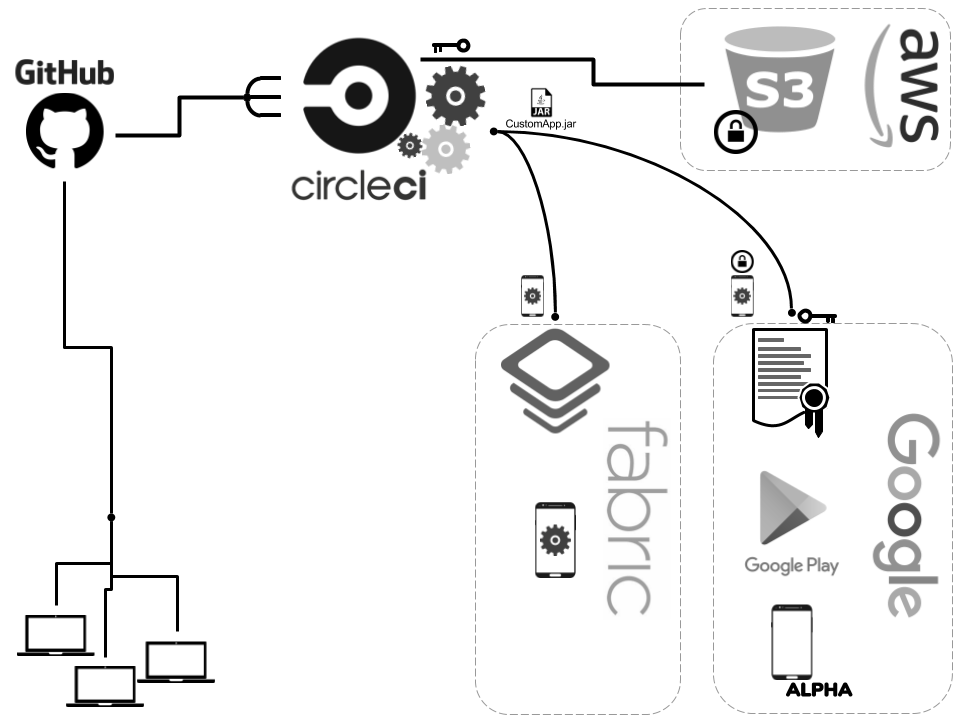
\includegraphics[width=0.9\textwidth]{Images/CICDFINAL.png}
\end{figure}	
\newpage
\section{Development tools}
In order to manage this project i used different development tools and Source Control tools. This was very useful as it enables working on different branches for features that i want to implement and leaves the master branch as a working state of the project. This could be used for industry standard as continuous delivery. For this project it's meant that after each sprint there was a working version to present to the customer. Although the working version does not mean it doesn't need changes in next sprints. I was solo this project so i did not take advantage of branches as much as a group would, as each member would have there own branch to work on.

\subsection{Android Studio}
Android Studio is the official integrated development environment (IDE) for Google's Android operating system, built on JetBrains' IntelliJ IDEA software and designed specifically for Android development. It is available for download on Windows, macOS and Linux based operating systems.It is a replacement for the Eclipse Android Development Tools (ADT) as the primary IDE for native Android application development.\newline
The integration between Android Studio and Firebase made Android Studio the most superior development platform to use.

\subsection{Firebase}
Firebase  is  Google’s  mobile  and  web  application  development  platform  that helps you build,  improve,  and grow your application.  Firebase frees developers to focus on crafting excellent user experiences.  You don’t need to manage servers.  You don’t need to write APIs.  Firebase is your server, your API and your database, everything is written generically so that you can modify every-thing  to  suit  most  needs.   

\section{Source Control}

\subsection{GitHub}
Github provides hosting for software development version control using Git. It offers the distributed version control and source code management (SCM) functionality of Git, plus its own features. It provides access control and several collaboration features such as bug tracking, feature requests, task management, and wikis for every project. GitHub offers plans free of charge, and professional and enterprise accounts. The Github kanban board was a feature i used in this project to track sprints.

\subsection{Overleaf}
Overleaf is an open-source online real-time collaborate LaTeX editor. It is hosted at http://www.overleaf.com, but can also run on your own local version, and contribute to the development of Overleaf.
\subsection{Badge/Shield}
Badge/Shield.io is a service for concise, consistent, and legible badges in SVG and raster format, which can easily be included in GitHub READMEs or any other web page. The service supports dozens of continuous integration services, package registries, distributions, app stores, social networks, code coverage services, and code analysis services. Every month it serves over 470 million images. \cite{badges}
This is used for easy access to a copy of the APK and Dissertation at the top of my README, you can further customize these badges to show Beta versions, stable versions, downloads, ratings, code coverage etc.

